\paragraph{Sơ đồ tuần tự luồng Pha Gateway gửi callback/IPN và Payment Service xác minh giao dịch}

Luồng nghiệp vụ này mô tả
phần đầu của callback/IPN sau khi User thao tác thanh toán trên Payment Gateway. Payment Service nhận callback public, xác minh chữ ký qua Payment Gateway Selector, đối chiếu transaction theo \texttt{txnRef}, kiểm tra số tiền và trạng thái hiện tại. Nếu transaction đang \texttt{pending} và thanh toán thành công, luồng chuyển sang pha 3 để cập nhật transaction, subscription và outbox.

\begin{figure}[H]
\centering
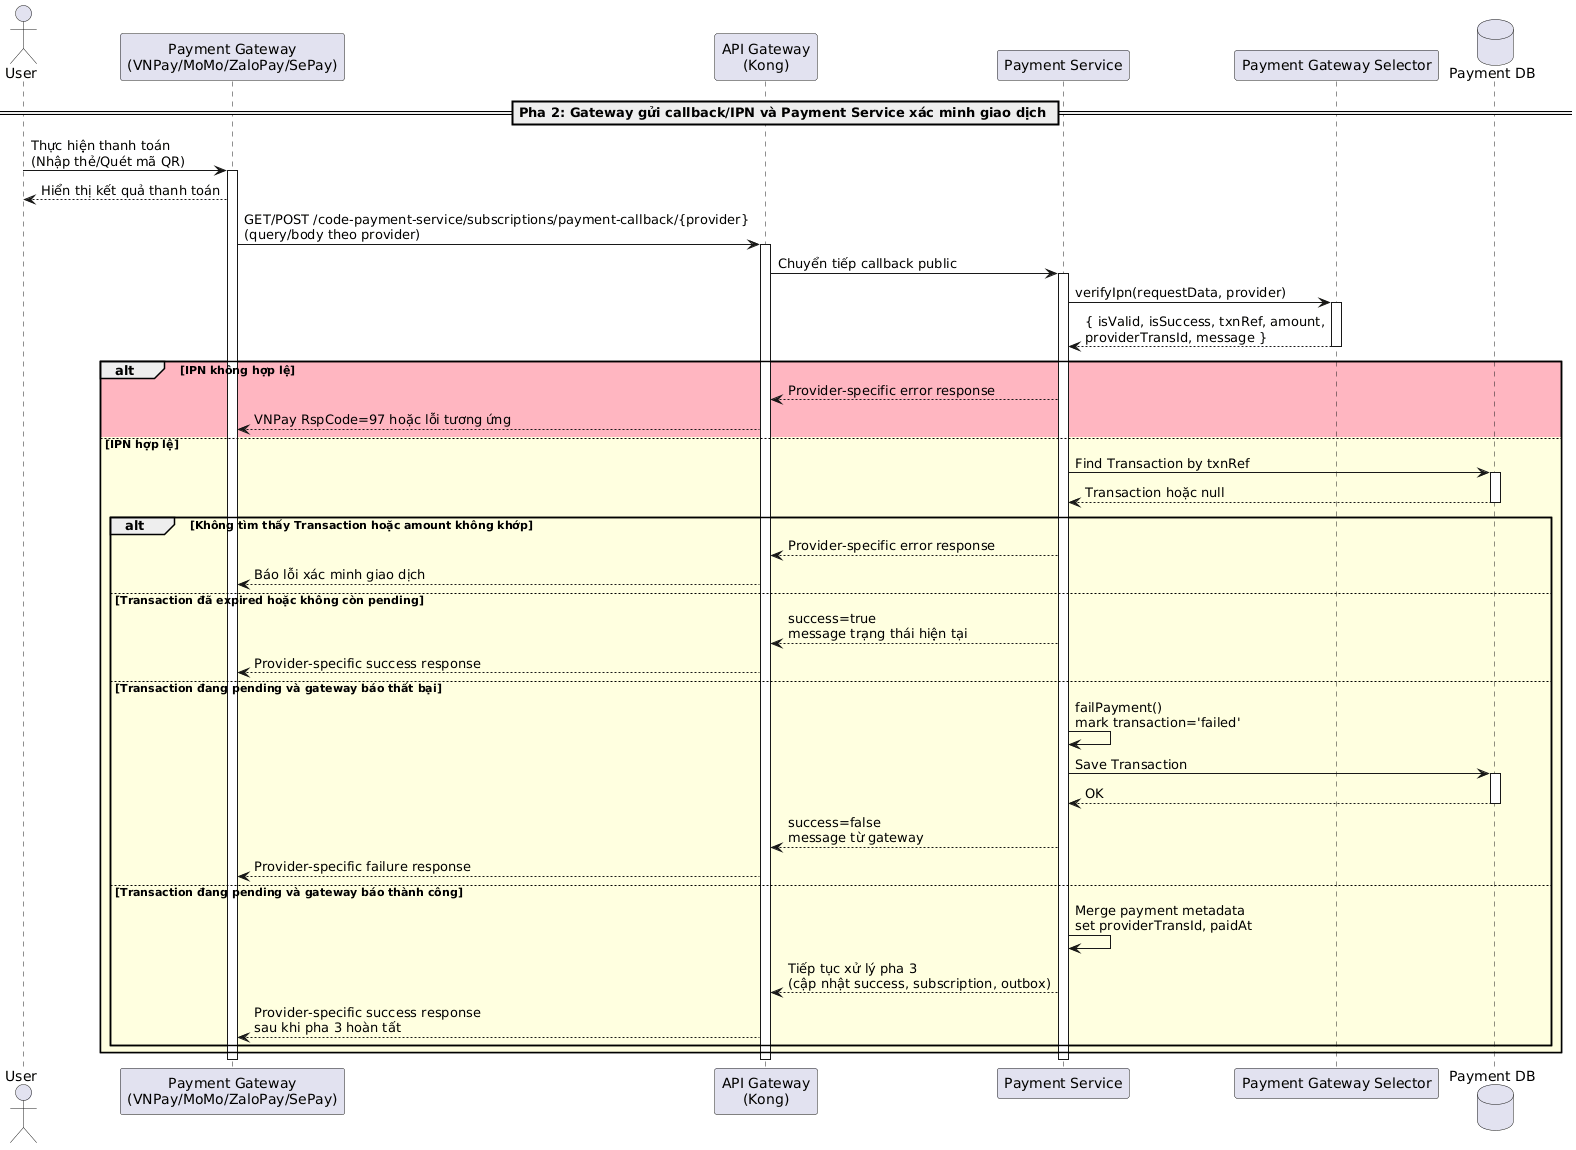
\includegraphics[scale = 0.2]{contents/Sequence/UML-Sequence-PaymentGatewayCallbackVerification.png}
\caption{Sơ đồ tuần tự luồng Pha Gateway gửi callback/IPN và Payment Service xác minh giao dịch}
\end{figure}

\subparagraph{Các thành phần tham gia}

\begin{table}[H]
\centering
\renewcommand{\arraystretch}{1.3}

\begin{tabular}{|l|l|p{5cm}|}
\hline
\textbf{Thành phần} & \textbf{Phân loại} & \textbf{Vai trò trong hệ thống} \\ \hline
User & Actor & Người dùng thực hiện thao tác thanh toán qua thẻ, ví điện tử hoặc mã QR trên Payment Gateway. \\ \hline
Payment Gateway & External Service & Xử lý thao tác thanh toán và gửi callback/IPN về hệ thống. \\ \hline
API Gateway (Kong) & Component & Cổng API chuyển tiếp các yêu cầu API. \\ \hline %%%% Component & Định tuyến callback public tới Payment Service qua endpoint của \texttt{code-payment-service}. \\ \hline
Payment Service & Microservice & Tiếp nhận callback, xác minh IPN, kiểm tra transaction, xử lý nhánh lỗi/thất bại hoặc chuyển tiếp sang pha cập nhật thành công. \\ \hline
Payment Gateway Selector & Component & Chọn adapter tương ứng. \\ \hline
Payment DB & Database & Cung cấp transaction cần đối chiếu bằng \texttt{txnRef}. \\ \hline
\end{tabular}
\caption{Các thành phần tham gia luồng pha Gateway gửi callback/IPN}
\end{table}

\subparagraph{Mô tả tổng quan}

\begin{itemize}

\item \textbf{Nhận thông báo thanh toán:}
Cổng thanh toán gửi thông tin phản hồi kết quả giao dịch về hệ thống.

\item \textbf{Đọc kết quả:}
Dịch vụ thanh toán chuyển yêu cầu cho bộ phận xử lý cổng thanh toán tương ứng để đọc kết quả phản hồi.

\item \textbf{Đối chiếu giao dịch:}
Dịch vụ kiểm tra tính hợp lệ của chữ ký giao dịch, đối chiếu mã giao dịch và số tiền thanh toán thực tế với thông tin giao dịch trong hệ thống. Nếu chữ ký không hợp lệ, không tìm thấy giao dịch hoặc số tiền không khớp, hệ thống trả về thông báo lỗi cho cổng thanh toán. Nếu giao dịch đã hết hạn hoặc không ở trạng thái chờ thanh toán, dịch vụ bỏ qua không xử lý lại.

\item \textbf{Xử lý thất bại:}
Nếu phản hồi hợp lệ nhưng cổng thanh toán báo giao dịch thất bại, dịch vụ chuyển trạng thái giao dịch trong hệ thống thành thất bại, lưu thông tin giao dịch và phản hồi kết quả lỗi cho phía cổng thanh toán.

\item \textbf{Xử lý thành công:}
Nếu phản hồi hợp lệ, giao dịch đang ở trạng thái chờ và cổng thanh toán báo thành công, dịch vụ lưu trữ thông tin giao dịch tạm thời và chuyển sang bước tiếp theo để hoàn tất cập nhật giao dịch, kích hoạt gói thuê bao VIP và phát sự kiện hệ thống.
\end{itemize}
